% 图 23.2 —— 由 `checks/emit_hand.py` 自动拼出（probe 精测 + prims2 图元分解）
%%
% ⚠ 这是**稿子不是成品**：跑 `checks/checkhand.py 23.2` 看指标 + 看叠合图。
%%
%% ⚠ 待核：
%   · 本图 probe 报出阴影族 1 个 —— **本脚本不生成阴影**（要照原书手写）；prims2 的 strokes 里可能含阴影线，核对时留意别画重
%   · 可疑字形 1 项（空心圈 ⊙ 常被认成字母 o）—— 见文件末
%%
\documentclass[12pt]{standalone}
\usepackage{fontspec}
\setsansfont{Arial}
\newfontfamily\mfallback{DejaVu Sans}
\usepackage{tikz}
\begin{document}
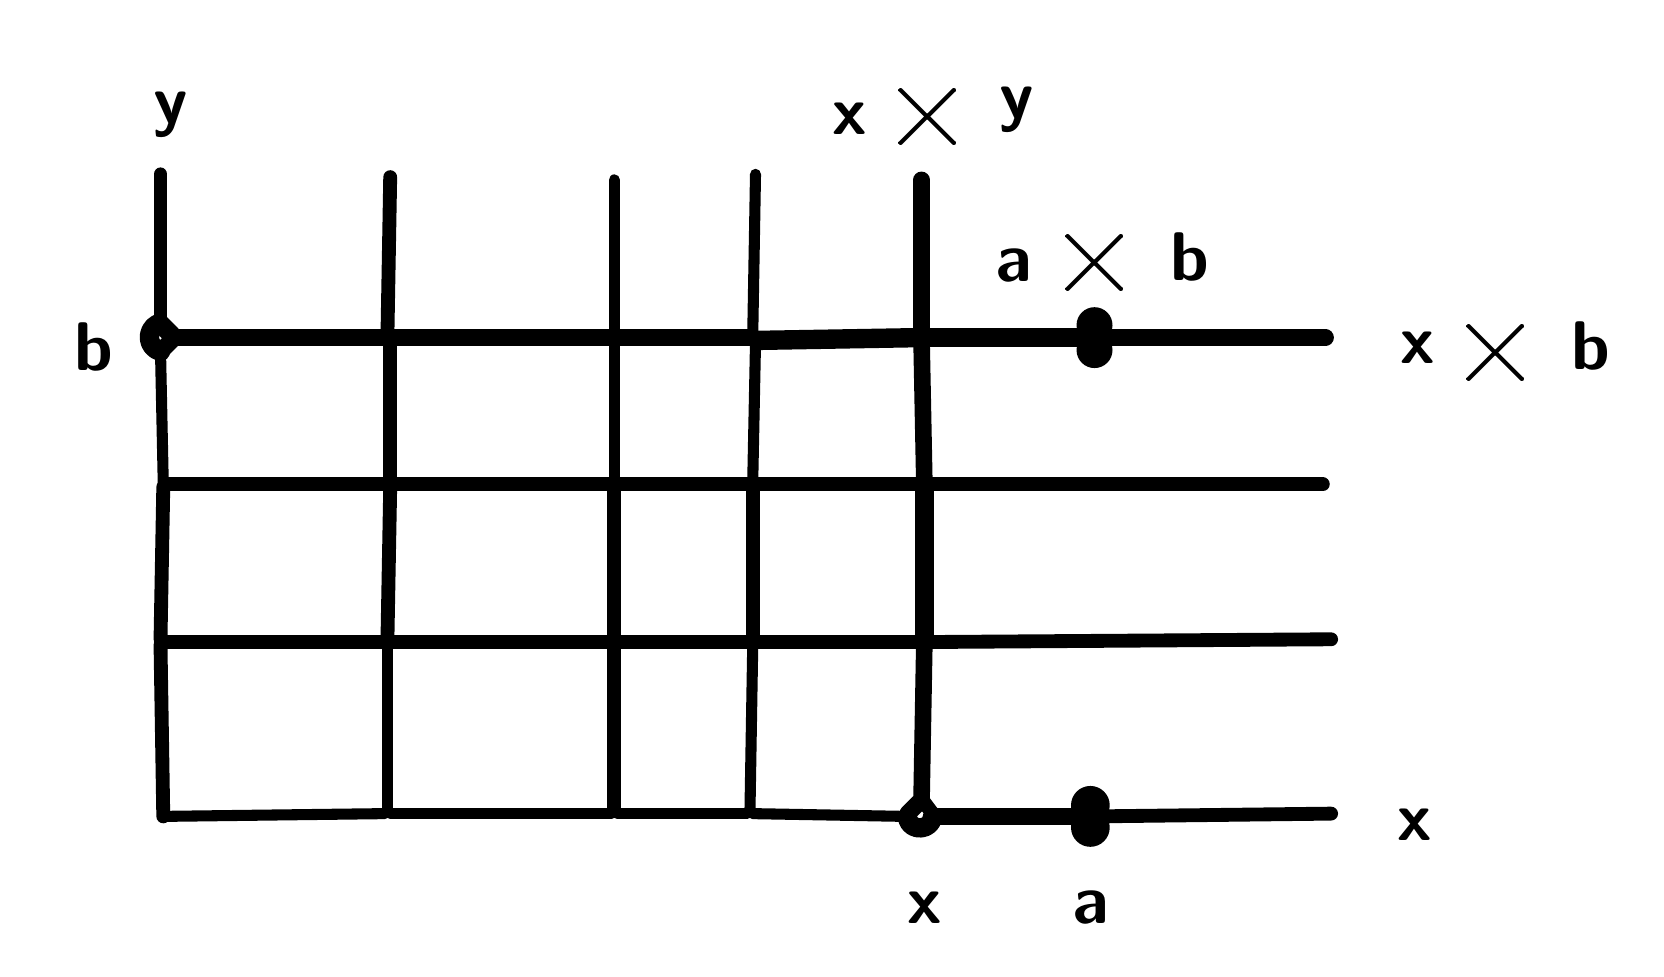
\begin{tikzpicture}[x=1pt, y=-1pt, line width=6.1pt, line cap=round, line join=round]

  %% ════ 填充区（prims2 的 fills）════

  %% ════ 直线段（prims2 的 strokes）════
  \draw[line width=6.1pt] (322.0,280.0) -- (318.0,284.0);
  \draw[line width=5.0pt] (213.0,222.0) -- (261.0,222.0);
  \draw[line width=7.0pt] (384.0,112.0) -- (324.0,112.0);
  \draw[line width=6.0pt] (324.0,223.0) -- (323.0,279.0);
  \draw[line width=4.0pt] (212.0,55.0) -- (212.0,111.0);
  \draw[line width=7.0pt] (322.0,112.0) -- (264.0,113.0);
  \draw[line width=5.0pt] (325.0,222.0) -- (471.0,221.0);
  \draw[line width=5.1pt] (324.0,280.0) -- (327.0,284.0);
  \draw[line width=6.0pt] (386.0,112.0) -- (469.0,112.0);
  \draw[line width=4.0pt] (263.0,53.0) -- (262.0,111.0);
  \draw[line width=4.0pt] (261.0,283.0) -- (262.0,223.0);
  \draw[line width=6.0pt] (132.0,112.0) -- (211.0,112.0);
  \draw[line width=5.0pt] (131.0,113.0) -- (131.0,164.0);
  \draw[line width=5.0pt] (48.0,221.0) -- (49.0,166.0);
  \draw[line width=5.0pt] (211.0,165.0) -- (132.0,165.0);
  \draw[line width=5.0pt] (386.0,285.0) -- (471.0,284.0);
  \draw[line width=5.0pt] (263.0,222.0) -- (323.0,222.0);
  \draw[line width=6.0pt] (323.0,113.0) -- (324.0,164.0);
  \draw[line width=5.0pt] (130.0,221.0) -- (131.0,166.0);
  \draw[line width=4.0pt] (49.0,165.0) -- (48.0,117.0);
  \draw[line width=6.1pt] (48.0,117.0) -- (52.0,113.0);
  \draw[line width=5.0pt] (212.0,223.0) -- (212.0,283.0);
  \draw[line width=5.0pt] (48.0,53.0) -- (48.0,106.0);
  \draw[line width=4.0pt] (262.0,284.0) -- (317.0,285.0);
  \draw[line width=5.0pt] (323.0,165.0) -- (263.0,165.0);
  \draw[line width=5.0pt] (261.0,165.0) -- (213.0,165.0);
  \draw[line width=5.0pt] (325.0,165.0) -- (468.0,165.0);
  \draw[line width=6.7pt] (48.0,107.0) -- (52.0,111.0);
  \draw[line width=5.0pt] (131.0,54.0) -- (130.0,111.0);
  \draw[line width=4.0pt] (130.0,283.0) -- (130.0,223.0);
  \draw[line width=4.0pt] (129.0,284.0) -- (49.0,285.0);
  \draw[line width=5.0pt] (49.0,285.0) -- (48.0,223.0);
  \draw[line width=6.0pt] (129.0,112.0) -- (53.0,112.0);
  \draw[line width=6.0pt] (328.0,285.0) -- (382.0,285.0);
  \draw[line width=4.0pt] (211.0,284.0) -- (131.0,284.0);
  \draw[line width=4.0pt] (212.0,164.0) -- (212.0,113.0);
  \draw[line width=6.0pt] (323.0,55.0) -- (323.0,111.0);
  \draw[line width=5.0pt] (212.0,166.0) -- (212.0,221.0);
  \draw[line width=4.0pt] (213.0,284.0) -- (260.0,284.0);
  \draw[line width=7.0pt] (324.0,166.0) -- (324.0,221.0);
  \draw[line width=6.0pt] (261.0,112.0) -- (213.0,112.0);
  \draw[line width=4.0pt] (262.0,164.0) -- (263.0,114.0);
  \draw[line width=5.0pt] (50.0,165.0) -- (130.0,165.0);
  \draw[line width=5.0pt] (262.0,166.0) -- (262.0,221.0);
  \draw[line width=5.0pt] (129.0,222.0) -- (49.0,222.0);
  \draw[line width=5.0pt] (211.0,222.0) -- (131.0,222.0);

  %% ════ 曲线（prims2 的 curves —— 三段式，坐标同为 (y,x)）════
  \draw[line width=7.0pt] (48.0,117.0) .. controls (43.2,115.7) and (42.5,109.4) .. (47.0,107.0);
  \draw[line width=7.0pt] (318.0,286.0) .. controls (319.4,290.8) and (326.8,289.9) .. (327.0,285.0);

  %% ════ 实心点 ════
  \fill (385.5,107.5) circle (6.5);
  \fill (385.5,116.5) circle (6.5);
  \fill (384.0,281.0) circle (7.0);
  \fill (384.0,289.0) circle (7.0);

  %% ════ 标签（probe 直接给的 \node 行）════
  %% ⚠ 全部补了 fill=white：文字在最上层，否则与曲线交叉干扰
     \node[anchor=center,inner sep=0pt,fill=white,font=\fontsize{29.2}{36.4}\selectfont] at (357.7,29.7) {\textsf{\textbf{\textit{y}}}};   % box(349,17,17,22)
     \node[anchor=center,inner sep=0pt,fill=white,font=\fontsize{28.5}{35.6}\selectfont] at (51.7,31.2) {\textsf{\textbf{\textit{y}}}};   % box(43,19,17,21)
     \node[anchor=center,inner sep=0pt,fill=white,font=\fontsize{30.1}{37.6}\selectfont] at (297.0,33.0) {\textsf{\textbf{\textit{x}}}};   % box(288,22,16,18)
     \node[anchor=center,inner sep=0pt,fill=white,font=\fontsize{33.8}{42.3}\selectfont] at (325.1,32.5) {\textsf{\textbf{×}}};   % box(317,22,15,16)
     \node[anchor=center,inner sep=0pt,fill=white,font=\fontsize{30.7}{38.3}\selectfont] at (419.8,82.8) {\textsf{\textbf{\textit{b}}}};   % box(410,70,17,23)
     \node[anchor=center,inner sep=0pt,fill=white,font=\fontsize{33.8}{42.3}\selectfont] at (385.6,85.0) {\textsf{\textbf{×}}};   % box(377,75,16,15)
     \node[anchor=center,inner sep=0pt,fill=white,font=\fontsize{31.0}{38.7}\selectfont] at (356.5,86.0) {\textsf{\textbf{\textit{a}}}};   % box(348,76,15,17)
     \node[anchor=center,inner sep=0pt,fill=white,font=\fontsize{37.2}{46.5}\selectfont] at (502.2,115.5) {\textsf{\textbf{\textit{x}}}};   % box(491,102,20,22)
     \node[anchor=center,inner sep=0pt,fill=white,font=\fontsize{30.7}{38.3}\selectfont] at (564.8,114.8) {\textsf{\textbf{\textit{b}}}};   % box(555,102,17,23)
     \node[anchor=center,inner sep=0pt,fill=white,font=\fontsize{30.0}{37.5}\selectfont] at (23.8,115.2) {\textsf{\textbf{\textit{b}}}};   % box(14,103,17,22)
     \node[anchor=center,inner sep=0pt,fill=white,font=\fontsize{34.9}{43.6}\selectfont] at (530.6,117.6) {\textsf{\textbf{×}}};   % box(522,107,16,16)
     \node[anchor=center,inner sep=0pt,fill=white,font=\fontsize{38.0}{47.5}\selectfont] at (501.3,288.0) {\textsf{\textbf{\textit{x}}}};   % box(490,274,20,23)
     \node[anchor=center,inner sep=0pt,fill=white,font=\fontsize{30.1}{37.6}\selectfont] at (324.0,318.0) {\textsf{\textbf{\textit{x}}}};   % box(315,307,16,18)
     \node[anchor=center,inner sep=0pt,fill=white,font=\fontsize{31.0}{38.7}\selectfont] at (384.5,318.0) {\textsf{\textbf{\textit{a}}}};   % box(376,308,15,17)

  % 钉死画布：否则超出的图元/控制点会把页面撑大，1:1 回比就失准
  \pgfresetboundingbox
  \path[use as bounding box] (0,0) rectangle (581,333);
\end{tikzpicture}
\end{document}

% ⚠ 待核清单（probe 拿不准，人眼过一遍）：
%   · 未识别/跳过：⑤ 跳过/未识别的字形
